\chapter{The \acl Algorithm} \label{sect:acl}
We now present our proposed \fullacl (\acl) algorithm for the strictly
sequential setting with explicit thresholds.
\acl is similar in spirit to the \gpucb~\cite{srinivas10}
bandit optimization algorithm in that it uses a GP to model the
underlying function and facilitates the inferred mean and variance of the GP
to guide the selection of points to be evaluated.

\begin{figure}[t]
  \begin{subfigure}[b]{0.49\linewidth}
    \centering
    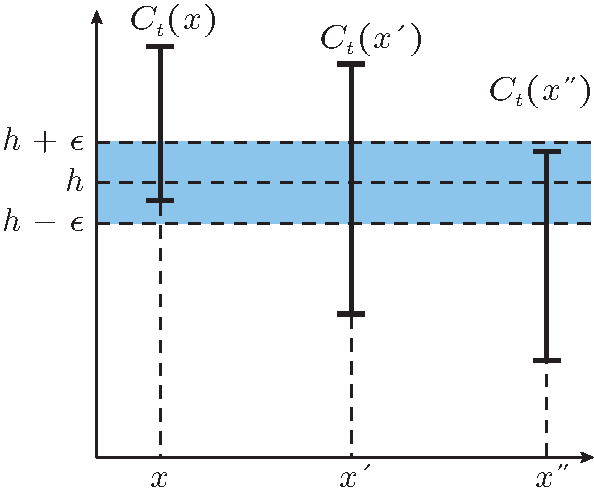
\includegraphics[height=1.4in]{figures/class}
    \caption{}
    \label{fig:conf}
  \end{subfigure}
  \hfill
  \begin{subfigure}[b]{0.49\linewidth}
    \centering
    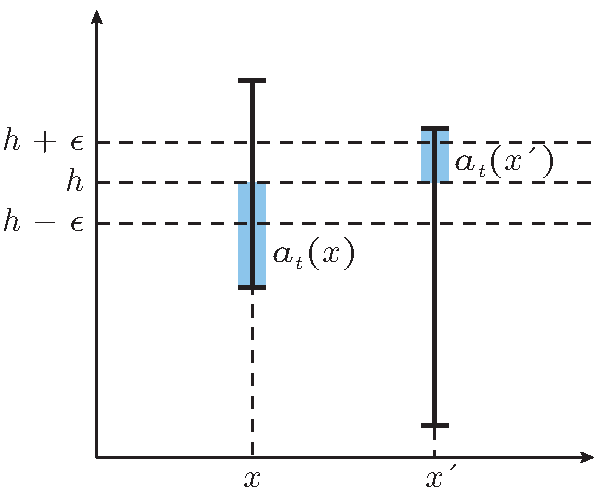
\includegraphics[height=1.4in]{figures/amb}
    \caption{}
    \label{fig:amb}
  \end{subfigure}
  \caption{
  (a) Example of the three possible configurations of confidence regions.
  (b) Ambiguities (shaded) of two example points.
  }
\end{figure}

More concretely, the inferred mean and variance of \eqtref{eq:mean}
and \eqtref{eq:var} can be used to construct a \emph{confidence interval}
\begin{align*}
Q_t(\*x) = \left[\mu_{t-1}(\*x) \pm \beta_t^{1/2}\sigma_{t-1}(\*x)\right]
\end{align*}
for any point $\*x \in D$, which captures our uncertainty about $f(\*x)$
after having already obtained noisy evaluations of $f$ at points
$\{\*x_1,\ldots,\*x_t\}$. The parameter $\beta_t$ acts as a scaling factor
and its choice is discussed later.
The above-defined confidence intervals serve two purposes in our algorithm:
first, they allow us to judge whether a point can be classified into
the super- or sublevel sets or whether the decision should be deferred
until more information is available; second, they guide the sampling
process towards points that are likely to be informative with respect
to the desired level set.

The pseudocode of \algoref{alg:acl} depicts in detail the operation of \acl.
Our algorithm maintains a set of yet unclassified
points $U_t$, as well as a superlevel set $H_t$ and a sublevel set
$L_t$, which are updated at each iteration. Furthermore, the algorithm
maintains for each $\*x$ a monotonically decreasing \emph{confidence
region} $C_t(\*x)$, which results from intersecting successive
confidence intervals, i.e.
\begin{align*}
C_t(\*x) = \bigcap_{i=1}^t Q_i(\*x) = C_{t-1}(\*x) \cap Q_t(\*x).
\end{align*}
Initially, all points
$\*x \in D$ are unclassified and the confidence regions have infinite
range (\linesref{lin:init1}{lin:init2}). At each iteration, the confidence
regions of all
unclassified points are updated (\lineref{lin:upd}) and each of these points
is either classified into one of $H_t$ or $L_t$, or is left unclassified
(\linesref{lin:class1}{lin:class2}). Then, the next point is selected and
evaluated (\linesref{lin:sel1}{lin:sel2}) and the new GP posterior is computed
(\lineref{lin:inf}). The algorithm terminates when all points in $D$ have been
classified, in which case the estimated super- and sublevel sets $\hat{H}$ and
$\hat{L}$ are returned (\linesref{lin:ret1}{lin:ret2}).

\begin{algorithm}[tb]
  \caption{The \acl algorithm}
  \label{alg:acl}
\small{
\begin{algorithmic}[1]
  \REQUIRE sample set $D$, GP prior ($\mu_0 = 0$, $k$, $\sigma_0$),\\
           \hspace{1.6em}threshold value $h$, accuracy parameter $\epsilon$
  \ENSURE predicted sets $\hat{H}$, $\hat{L}$
  \LET{$H_0$}{$\varnothing$} \label{lin:init1}
  \LET{$L_0$}{$\varnothing$}
  \LET{$U_0$}{$D$}
  \LET{$C_0(\*x)$}{$\mathbb{R}$, for all $\*x \in D$} \label{lin:init2}
  \LET{$t$}{1}
  \WHILE{$U_{t-1} \neq \varnothing$}
    \LET{$H_t$}{$H_{t-1}$}
    \LET{$L_t$}{$L_{t-1}$}
    \LET{$U_t$}{$U_{t-1}$} 
    \FORALL{$\*x \in U_{t-1}$}
      \LET{$C_{t}(\*x)$}{$C_{t-1}(\*x) \cap Q_t(\*x)$} \label{lin:upd}
      \IF{$\min(C_t(\*x)) + \epsilon > h$} \label{lin:class1}
        \LET{$U_t$}{$U_t \setminus \{\*x\}$}
        \LET{$H_t$}{$H_t \cup \{\*x\}$} 
      \ELSIF{$\max(C_t(\*x)) - \epsilon \leq h$} \label{lin:classr2}
        \LET{$U_t$}{$U_t \setminus \{\*x\}$}
        \LET{$L_t$}{$L_t \cup \{\*x\}$}
      \ENDIF \label{lin:class2}
    \ENDFOR
    \LET{$\*x_t$}{$\argmax_{\*x \in U_t}(a_t(\*x))$} \label{lin:sel1}
    \LET{$y_t$}{$f(\*x_t) + \nu_t$} \label{lin:sel2}
    \STATE Compute $\mu_t(\*x)$ and $\sigma_t(\*x)$, for all $\*x \in U_t$ \label{lin:inf}
    \LET{$t$}{$t + 1$}
  \ENDWHILE
  \LET{$\hat{H}$}{$H_{t-1}$} \label{lin:ret1}
  \LET{$\hat{L}$}{$L_{t-1}$} \label{lin:ret2}
\end{algorithmic}
}
\end{algorithm}

We now discuss in more detail the issues of how points are classified and
how the next point is selected at each step.

\paragraph{Classification}
The classification of a point $\*x$ into $H_t$ or $L_t$ depends on the
position of its confidence region with respect to the threshold level $h$.
Intuitively, if all of $C_t(\*x)$ lies above $h$, then with high probability
$f(\*x) > h$ and $\*x$ should be moved into $H_t$. Similarly, if $C_t(\*x)$
lies below $h$, then $\*x$ should be moved into $L_t$. Otherwise, we are
still uncertain about the class of $\*x$, therefore it should, for the moment,
remain unclassified. As can be seen in the classification rules
of~\linsref{lin:class1} and~\ref{lin:classr2}, we relax these conditions by
introducing an accuracy parameter $\epsilon$, which
trades off classification accuracy for sampling cost. The resulting
classification scheme is illustrated by the example of \figref{fig:conf},
in which point $\*x$ would be
classified into $H_t$ and point $\*x''$ into $L_t$, while point $\*x'$ would
remain in $U_t$ as unclassified. Note that \acl uses a monotonic
classification scheme, meaning that once a point has been classified, it
stays so until the algorithm terminates.

\paragraph{Sample selection}
For selecting the next point to be evaluated at each iteration, we define the
following quantity
\begin{align*}
a_t(\*x) = \min\{\max(C_t(\*x)) - h, h - \min(C_t(\*x))\},
\end{align*}
which we call \emph{ambiguity}. As its name suggests, the ambiguity of a
point $\*x$ quantifies our uncertainty about whether $\*x$ belongs to
$H_t$ or $L_t$ (see \figref{fig:amb}).
The intuition of sampling at areas of the sample space with large
classification uncertainty, expecting to gain more information about
the problem at hand when sampling at those areas, manifests itself in \acl
by choosing to evaluate at each iteration the point with the largest
ambiguity amongst the yet unclassified
(see~\figsref{fig:limno_chl} and~\ref{fig:limno_chl_class}).

We can make an interesting observation at this point. If we use the confidence
intervals $Q_t(\*x)$ instead of the confidence regions $C_t(\*x)$
in the definition of ambiguity, we get
\begin{align*}
a'_t(\*x) &= \min\{\max(Q_t(\*x)) - h, h - \min(Q_t(\*x))\}\\
         &= \beta_t\sigma_{t-1}(\*x) - |\mu_{t-1}(\*x) - h|.
\end{align*}
For $\beta_t = 1.96$, this is identical to
the \emph{straddle}~\cite{bryan05} selection rule, which can thus be
intuitively explained in terms of classification ambiguity.

\paragraph{Theoretical analysis}
The convergence analysis of \acl rests on quantifying the complexity of the GP prior for $f$ in information-theoretic terms.
The information gain~\cite{cover06} about $f$ from observing $t$ noisy
measurements $\*y_t = (y_i)_{1\leq i\leq t}$ is
\begin{align*}
I(\*y_t; f) = H(\*y_t) - H(\*y_t\mid f).
\end{align*}
\citet{srinivas10} used the \emph{maximum
information gain} over all possible sets of $t$ observations
\begin{align*}
\gamma_t = \max_{\*y_t} I(\*y_t; f)
\end{align*}
for bounding the regret of the \gpucb algorithm.
We use the same quantity to bound the number of \acl iterations
required to achieve a certain classification quality.

To quantify the quality of a solution $(\hat{H}, \hat{L})$
with respect to a single point $\*x\in D$ we use the
misclassification loss
\begin{align*}
\ell_h(\*x) = \twopartdef{\max\{0, f(\*x) - h\}}{\*x\in \hat{L}}{\max\{0, h - f(\*x)\}}{\*x\in \hat{H}}.
\end{align*}
The overall quality of a solution can then be judged by the
largest misclassification loss
among all points in the sample space, i.e. $\max_{\*x\in D} \ell_h(\*x)$.
Intuitively, having a solution with $\max_{\*x\in D} \ell_h(\*x) \leq \epsilon$
means that every point $\*x$ is correctly classified with respect to a
threshold level that deviates by at most $\epsilon$ from the true level $h$;
we call such a solution \emph{$\epsilon$-accurate}.
The following theorem establishes a convergence bound for \acl in terms
of $\gamma_t$ for any given accuracy $\epsilon$.

\begin{theorem}
\label{thm:acl}
For any $h\in\mathbb{R}$, $\delta \in (0, 1)$, and $\epsilon > 0$,
if $\beta_t = 2\log(|D|\pi^2 t^2/(6\delta))$, \acl terminates after
at most $T$ iterations, where $T$ is the smallest positive integer
satisfying
\begin{align*}
\frac{T}{\beta_T \gamma_T} \geq \frac{C_1}{4\epsilon^2},
%T/(\beta_T \gamma_T) \geq C_1/(4\epsilon^2),
\end{align*}
where $C_1 = 8/log(1 + \sigma^{-2})$.

Furthermore, with probability at least $1-\delta$, the algorithm returns
an $\epsilon$-accurate solution, that is
\begin{align*}
\Pr\left\{\max_{\*x\in D}\ell_h(\*x) \leq \epsilon\right\} \geq 1 - \delta.
\end{align*}
\end{theorem}

The proof of \theoremref{thm:acl} can be
outlined as follows.\footnote{Detailed proofs of all theorems and further
experiments can be found in the supplemental material of this paper
(\url{http://sites.google.com/site/lseijcai13/long.pdf}).}
The choice of $\beta_t$ guarantees
the inclusion of $f(\*x)$ in the confidence regions $C_t(\*x)$ for
all $\*x\in D$. From the monotonic classification scheme and
the maximum ambiguity selection rule, it follows that the
ambiguities of the selected points, $a_t(\*x_t)$, are decreasing
with $t$ and, using $\gamma_t$, they can be shown to decrease
as $\mathcal{O}((\frac{\beta_t \gamma_t}{t})^\frac{1}{2})$. Finally,
the classification rules of \acl connect the number of iterations to
the accuracy parameter $\epsilon$ and guarantee an $\epsilon$-accurate
solution with high probability.

Note that bounds on $\gamma_t$ have been established for commonly used
kernels~\cite{srinivas10} and can be plugged into \theoremref{thm:acl}
to obtain concrete bounds on $T$.
For example, for a \mbox{$d$-dimensional} sample space and a squared exponential
GP kernel, ${\gamma_t = \mathcal{O}((\log T)^{d+1})}$, and the expression in
the bound of
\theoremref{thm:acl} becomes $T/(\log T)^{d+2} \geq C / \epsilon^2$,
where, for any given sample space and kernel hyperparameters, $C$ depends
only on the choice of $\delta$.